\documentclass[main.tex]{subfiles}
\newcommand{\snzi}{\sum_{n=0}^{+\infty}}
\newcommand{\snii}{\sum_{n=0}^{+\infty}}

\begin{document}
\section{Généralités}

Les filtres à capacités commutées sont un premier exemple de filtres échantillonnés pouvant être intégrés sur une technologie CMOS mais comportent encore des parties analogiques avec des possibilités limitées pour la conception des filtres.

L'idée est de réaliser entièrement les opérations de filtrage par un traitement numérique sur processeur CMOS. (DSP : digital signal processing)

\begin{figure}[H]
  \centering
  \begin{tikzpicture}
    \draw (0,0)node[below left]{$x_c(t)$}to[short,o-] ++(1,0)to[spst] ++(2,0) coordinate (E) to[C] ++(0,-2) node[ground]{};
    \draw[dashed] (1,1) rectangle (4,-2) (2.5,1){node[above]{Echantilloneur bloqueur}} ;
    \sbBlocL{can}{CAN}{E}
    \sbBlocL{F}{
      \begin{tabular}{c}
Filtre \\linéaire
      \end{tabular}
    }{can}
    \sbBlocL{cna}{CNA}{F}
    \draw (cna) -- ++(1,0) to[lowpass,-o] ++(2,0) node[below right]{$y_c(t)$};
  \end{tikzpicture}
  \caption{Principe d'un filtre numérique}
\end{figure}

avec \[y_E(nT_e) = \sum_{m=-\infty}^{+\infty} h(nT_e) x((n-m)T_e)\]
où $h(mT_e)$ est la réponse impulsionnelle du filtre et la somme de $-\infty$ à $+\infty$ traduit le fait que le filtre n'est pas forcément causal. Si le filtre n'est pas causal, on a des retards systématiques de $kT_e$, $k$ entiers, entre l'entrée et la sortie. \\

On utilise par la suite des notations simplifiées :
\begin{align*}
y(n) & = \sum_{m=-\infty}^{+\infty} h(m) x(n-m) \\
y(n) & = \sum_{m=-\infty}^{+\infty} h(n-m) x(m)
\end{align*}

\noindent \textbf{Idée :} programmer (réaliser) l'ensemble des calculs nécessaires sur un circuit numérique, après conversion analogique / numérique (CAN).\\

\textbf{Intérêts :}
\begin{itemize}
\item améliorer le rapport signal à bruit
\item profiter de la puissance des circuits CMOS : aujourd'hui, circuits à quelques milliards de transistors à un prix raisonnable (ULSI : ultra large scale integration) grâce à la réduction progressive de la longueur de grille $L_G$ en fonction des années (de \SI{0.1}{\micro\meter} en 1971 à \SI{30}{nm} ou un peu moins actuellement)
\item grande diversité possible pour la conception des filtres, avec une faible variabilité sur les caractéristiques des circuits, avec une grande vitesse de calcul
\end{itemize}

\textbf{Défauts :}
\begin{itemize}
\item respecter Shannon (vrai aussi pour les capacités commutées)
\item nécessité d'une horloge très stable (vrai aussi pour les capacités commutées)
\item Erreurs possibles sur les calculs à virgule flottante dans un DSP
\item Bruit de quantification (cf CAN)
\item Systèmes pas forcément en "temps réel"
\end{itemize}


\section{Caractéristiques des systèmes linéaires invariant dans le temps}

\subsection{Réponse impulsionnelle}
Pour le filtre linéaire suivant:
\[e_n \rightarrow \boxed{h} \rightarrow y_n = \sum_{m=-\infty}^{+\infty} h_m e_{n-m} \]
\begin{defin}
En utilisant une entrée impulsionnelle (impulsion de dirac):
\[ x_n = \begin{cases}
    1 & \text{si } n=0\\
    0 & \text{sinon}
    \end{cases}
  \]
  On obtient en sortie du filtre la \emph{réponse impulsionnelle:}
\[ y_n = h_n \]
\end{defin}
\subsection{Transformée en $z$}

\begin{align*}
y_E(nT_e) & = \sum_{m=-\infty}^{+\infty} h((n-m)T_e)x_E(mT_e) \\
& = (\sum_{m=-\infty}^{+\infty}h((n-m)T_e) \delta(t-(n-m)T_e)) * x_E(t) \quad (=h(t) * x_E(t))
                                                      \intertext{La transformée de Laplace de $\delta((n-m)T_e)$ est $\exp(p(n-m)T_e)=z^{n-m}$ où $z=\exp(pT_e)$}
\end{align*}
\begin{prop}[Transformée en Z]
On peux exprimer une signal discret par sa transformée en $Z$ , analogue à la transformée de Laplace:
\[
Y(z)  = H(z)X(z) \quad \text{ avec } H(z) = \sum_{m=-\infty}^{+\infty} h_mz^{-m}
\]
\end{prop}
\begin{rem}
Une multiplication par $z^{-1}$ correspond à un retard de $T_e$ sur le signal
\end{rem}

\subsection{Gain complexe}
\newcommand{\omegab}{\overline{\omega}}
\begin{align*}
H(e^{j\omega T_e}) & = \sum_{m=-\infty}^{+\infty} h_m \exp(-jm\omega T_e) \\
H(e^{j \omega_b}) & = \sum_{m=-\infty}^{+\infty} h_m \exp(-jm\omega_b) \quad \text{ avec } \omega_b = \omega T_e = 2 \pi fT_e
\end{align*}

\subsection{Causalité}
\[ y_n = \sum_{m=N_0}^{+\infty} h_m x_{n-m} \]

Si $N_0 \geq 0$, $y_n$ ne dépend que de $x_n$ et $x_m$ avec $m<n$ : filtre causal.

Si $N_0 < 0$, $y_n$ dépend aussi de $x_m$ avec $m>n$ : filtre non causal.\\

Un filtre numérique non causal est réalisable physiquement quand on accepte un retard systématique de $|N_0|T_e$ entre l'entrée et la sortie.

\subsection{Stabilité}

\begin{defin}
Un système est stable si et seulement si il présente une sortie qui reste finie quand l'entrée est finie, autrement dit : s'il existe $P>0$ tel que $\forall n, |x_n|<P$, alors il existe $Q>0$ tel que $\forall n, |y_n|<Q$.
\end{defin}

\paragraph{Conséquence sur la réponse impulsionnelle}
\begin{prop}
Un filtre numérique est stable si et seulement si $\sum_{n=-\infty}^{\infty} |h_n|$ est fini.
\end{prop}
\begin{proof}~
  \begin{itemize}
  \item Condition suffisante:

\[ |y_n| = |\sum_m h_m x_{n-m}| \leq \sum_m|h_m||x_{n-m}| \]
Si $|x_n|<l$ alors $|y_n| \leq P \sum_m |h_m|$ donc si $\sum_m |h_m|<R$, alors $|y_n| < PR$.\\

\item Condition nécessaire:

Soit $x_n =
\begin{cases}
  -1 \text{ si } h_{-n} < 0\\
  1 & \text{sinon}
\end{cases}$
(entrée finie)

Alors $y_0 = \sum_m h_m x_{0-m} = \sum_m h_{-m} x_m = \sum_m |h_m|$

$y_0$ doit rester fini donc $\sum_m |h_m|$ doit rester finie.

\end{itemize}
\end{proof}

\begin{prop}[Condition sur la transformée de Z]
Pour que le filtre soit stable les pôles $p_0$  de la transformée de Laplace de sa réponse impulsionnelle doivent être tels que $Re(p_0) < 0$.

Or, $z = \exp(pT_e)$ donc les pôles de $H(z)$ doivent être à l'intérieur (strictement) du cercle unité.
\end{prop}


\subsection{Différents types de filtres}
\begin{itemize}
\item À réponse impulsionnelle finie (RIF)

  cas où $h_n$ est nul pour $|n| > N_0$. Naturellement filtres stables.

\begin{exemple}[Calcul de la dérivée numérique d'un signal]
%\img{0.5}{3/2.png}

$\dd{x_c}{t}(nT_e)$ est proche de $y_n = \frac{x_E(nt_e)-x_E((n-1)T_e)}{T_e}$ si $T_e$ assez faible

Soit $y_n = \sum_m h_m x_{n-m}$ avec $h_0 = \frac{1}{T_e}, h_1 = -\frac{1}{T_e}, h_n = 0 si n\neq 0 \text{ ou } 1$

\begin{align*}
y_n & = h(0)x_n - h(1)x_{n-1} \\
& = \frac{1}{T_e} x_n - \frac{1}{T_e} x_{n-1} \\
Y(z) &= \frac{X(z)}{T_e} - \frac{X(z)}{T_e}z^{-1} \\
H(z) & = \frac{1-z^{-1}}{T_e}
\end{align*}
\begin{figure}[H]
  \centering
    \begin{tikzpicture}
    \begin{axis}
      [axis lines = middle, width=8cm,
      xmin=0,xmax = 10,ymin=-2,ymax=3,
      ytick =\empty, ylabel={{\color{blue}$x_c(t)$}, {\color{red}$x_E(t)$}},
      xtick = {3,6,9},xticklabels={$(n-1)T_e$,$n T_e$,$(n+1)T_e$},
      ytick = {1,-1.5},yticklabels={$x_E((n-1)T_e)$,$x_E(nT_e)$},
      x tick label style={yshift={mod(\ticknum,2)*1.5em}}]
      \addplot+[smooth,no marks] plot coordinates{(0,2) (2,1.5) (3,1) (4,1) (5,-1.5)(6,-1.5)(7,0)(9,1)};

      \addplot+[no marks, red, dashed] plot coordinates
      {(0,2) (3,1) (6,-1.5)};
    \end{axis}
  \end{tikzpicture}
  \caption{Echantillonneur bloqueur}
\end{figure}
\end{exemple}

\item À réponse impulsionnelle infinie (RII)

  il n'existe pas $N_0 > 0$ tel que $h_m=0$ pour $|n| > N_0$. Non nécessairement stable.

\begin{exemple}[Intégration numérique par la méthode des trapèzes]
$\int_{(n-1)T_e}^{nT_e} x(t)dt$ est proche de $T_e\frac{x_E((n-1)T_e)+x_E(nT_e)}{2}$. On peut procéder de façon récursive sur un grand nombre de périodes :

\begin{align*}
y_n & = y_{n-1} + \frac{x_{n-1}+x_n}{2}T_e \\
Y(z) & = z^{-1}Y(z) + \frac{T_e}{2} X(z)(1+z^{-1}) \\
H(z) & = \frac{T_e}{2} \frac{1+z^{-1}}{1-z^{-1}}
\end{align*}

On a aussi, si $|z| < 1$
\begin{align*}
H(z) &= \frac{T_e}{2}(1+z^{-1}) \sum_{n=0}^{+\infty} z^{-n} \\
H(z) &= \frac{T_e}{2} \snzi z^{-n} + \frac{T_e}{2} \snzi z^{-n-1} \\
H(z) &= \frac{T_e}{2} + T_e \sum_{n=1}^{+\infty} z^{-n}
\end{align*}
$h_0 = T_E/2$, $h_n=T_e$ si $n>0$ et $h_n=0$ si $n<0$\\

RII causale instable (récursif)
\end{exemple}
\end{itemize}
\section{Méthode de synthèse}

\paragraph{Cahier des charges}

programmation d'un filtre sur DSP sous la forme $y_n = \sum_m h_m x_{n-m}$ ou si le filtre est récursif par une équation aux différences du type $y_n = \sum_{m=-\infty}^{\infty} a_my_m + \sum_{m=-\infty}^{\infty} b_mx_m$ (causal)

$\rightarrow$ matérialisation simple en termes de calculs sur DSP notamment pour les filtres récursifs

\begin{exemple}
\[y_n = a_1y_{n-1} + b_0x_n + b_1x_{n-1} + b_2x_{n-2}\]

%\img{0.5}{4/1.png}
\end{exemple}

\subsection{Transposition d'un filtre à temps continu}

Le cahier des charges impose un gabarit $H_c(p)$ filtre à temps continu.

\[H_c(j\omega) = H_c(p=f(z)) = H_c(f(\exp(j\omega T_e))\]

où $f(z)$ doit conserver la stabilité (si $|z| < 1$, alors $Re(p=f(z))<0$).\\

On étudie ensuite $H(j\omega)$ afin de vérifier si elle vérifie bien le cahier des charges. Sinon, il faut réajuster des paramètres de $H_c$ ou le choix de la fonction de transposition.

\begin{exemple}[Transformée d'Euler] \[p=\frac{1-z^{-1}}{T_e}\]

Elle équivaut à $z = \frac{1}{1-pT_e}$.

\begin{itemize}
\item $H_c(p)$ est stable si ses pôles sont tels que $p_0=a+jb$ avec $a<0$ et $b\in \R$.

L'image de $p_0$ dans l'espace des $z$ est $z_0 = \frac{1}{1-aT_e -jbT_e}$ de module \[|z_0| = \frac{1}{\sqrt{(1-At_e)^2 + (bT_e)^2}} <1 \si a < 0\] La stabilité est conservée.

\item Vérifions dans quel domaine cette transformation est valable.\[ p = \frac{1-e^{-j\omega T_e}}{T_e} = e^{-j\omega T_e/2} \frac{2j}{T_e} \sin(\omega \frac{T_e}{2}) \text{ donc } |p| = \frac{2}{T_e}|\sin(\omega \frac{T_e}{2})| = \omega_a\]
Si $\omega \to 0$, $\omega_a \approx \omega$ donc $|H(j\omega)|$ et $|H_c(j\omega_a)|$ ont des comportements très proches

Pour $\omega$ plus grand, ce n'est plus vrai. Une distorsion apparaît entre $\omega$ et $\omega_a$ et augmente quand $\omega$ augmente. $|H_c(j\omega_a)|$ va avoir un comportement très différent de $|H-j\omega)|$.
%\img{0.5}{4/2}
%\img{0.5}{4/3}
\end{itemize}
\end{exemple}

\begin{exemple}[Transformée bilatère ou bilinéaire]
\[p=\frac{1}{\frac{1}{p}}=\frac{2}{T_e} \frac{1-z^{-1}}{1+z^{-1}}\]

Elle équivaut à $z=\frac{2+pT_e}{2-pT_e}$
\begin{itemize}
\item Soit $p_0=a+jb$ avec $a<0$ et $b\in \R$.

L'image de $p_0$ dans l'espace des $z$ a pour module \[ |z_0| = \sqrt{\frac{(2+aT_e)^2+(bT_e)^2}{(2-aT_e)^2+(bT_e)^2}} < 1 \si a < 0\]
La stabilité est conservée.

\item En remplaçant $z=\exp(j\omega T_e)$
\[ p = \frac{2}{T_e} j\tan(\omega \frac{T_e}{2}) = j\omega_a \]

Si $\omega \to 0$, $\omega_a \approx \omega$.

%\img{0.5}{4/4}
\end{itemize}
\end{exemple}

\subsection{Échantillonnage de la réponse impulsionnelle d'un filtre à temps continu}

\paragraph{Méthode brute}
\[ h_n = h_c(nT_e) \rightarrow y_n = \sum_{m=0}^{\infty} h_c(nT_e)x_{n-m}\]
Cette forme décrit un filtre causal mais avec une réponse impulsionnelle infinie.

\begin{exemple}[Filtre passe-bas d'ordre 1]

\begin{align*}
H_c & = \frac{A_0}{p-p_0} \text{ avec } Re(p_0) < 0 \\
h_c(t) & = A_0 \exp(p_0 t) \\
h_n & = A_0 \exp (p_0 nT_e) \\
H(z) & = A_0 \sum_{m=0}^{\infty} \exp(mp_0T_e)z^{-m} \\
& = \frac{A_0}{1-\exp(p_0T_e)z^{-1}}
\end{align*}
Pôle $z_0 = \exp(p_0T_e)$ avec $|z_0|=\exp(Re(p_0)T_e) < 1$
\end{exemple}

\paragraph{Méthode par fenêtrage} On pondère $h_c(nT_e)$ par une fenêtre $w(nT_e)$ de durée finie.

Soit $h_n=h_c(nT_e)w(nT_e)$ où $w(t)=0$ pour $|t| > T_0$ afin d'obtenir un filtre à réponse impulsionnelle finie.

\begin{exemple}[Fenêtrage rectangulaire]
  \[ w(t) = \begin{cases}
      1 & \text{ si } 0 \leq t \leq T_W = NT_e \\
      0 & \text{ sinon } \end{cases}
  \]
On a donc
\begin{align*}
  H(z) & = H_0(z) * w(z) \text{ où }
         \begin{cases}
           H_0(z) & = \sum_{n=0}^{\infty} h_c(nT_e)z^{-n} \text{ filtre RII précédent }\\
           w(z) & = \sum_{n=0}^N z^{-n}
       \end{cases}\\
w(z) & = \frac{1-z^{-(N+1)}}{1-z^{-1}}
\intertext{ Si $z=\exp(j\omegab)$ où $\omegab=\omega T_e$, alors }
w(\exp(j\omegab)) & = \exp(-jN\frac{\omegab}{2}) \frac{\sin(\frac{N+1}{2}\omegab)}{\sin(\frac{\omegab}{2})}
\end{align*}

Si $N>>1$ :
%\img{0.5}{4/5}

Conséquences sur $H(\exp(j\omegab))$ :
\begin{itemize}
\item apparition d'ondulations dans la réponse en fréquence la plus importante en amplitude correspondant à l'influence du lobe principale : phénomène de Gibbs, oscillations
\item dégradtion de la pente du filtre (pente plus faible à la coupure que pour le passe bas à temps continu prototype) d'autant plus grande que $N$ est faible
\end{itemize}
\end{exemple}

\begin{exemple}[Fenêtre de Hamming]
\[ w(nT_e) =
  \begin{cases}
    0.54 + 0.46\cos(\frac{2\pi n}{2N_0}) & \text{ si } |n| \leq N_0\\
    0 & \text{ sinon }
\end{cases}
\]

$|w(\exp(j\omegab))|$ a un lobe principal plus large que celui de la fenêtre rectangulaire mais des lobes secondaires plus faibles.

Il y a moins d'oscillations de Gibbs mais la pente est encore plus dégradée (réduction de la bande passante)
\end{exemple}

\begin{figure}[H]
  \begin{center}
    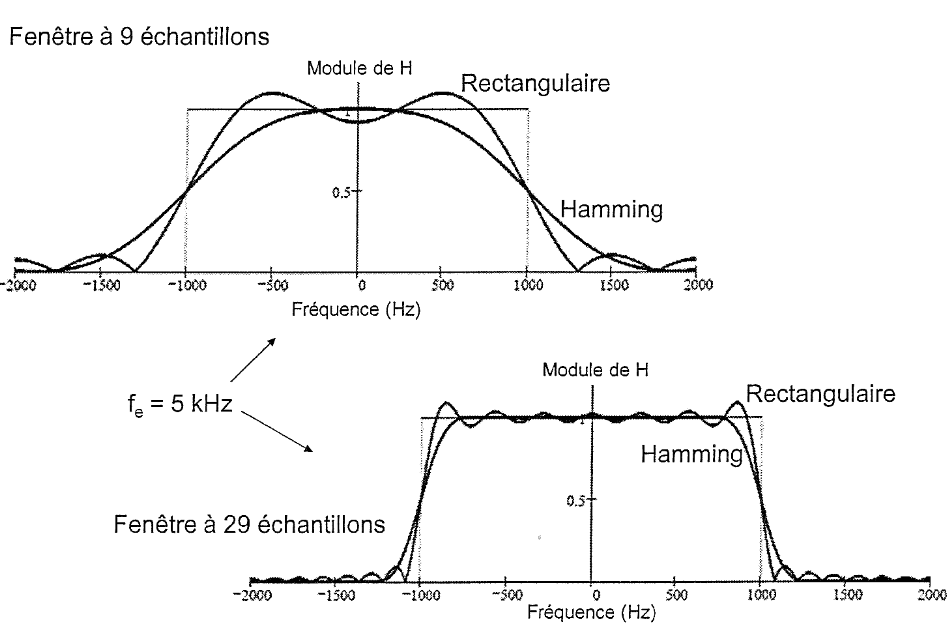
\includegraphics[width=0.9\textwidth]{poly}
    \caption{Représentation des fenêtres}
  \end{center}
\end{figure}

Pour caractériser les fenêtres, on utilise les paramètres suivants :
\begin{itemize}
\item Niveau de lobe secondaire : $N_S = 20\log(A_1/A_0)$ où $A_0$ amplitude du lobe principal et $A_1$ amplitude du lobe secondaire
\item FWHM : full width at half maximum ; largeur à mi hauteur du lobe principal
\end{itemize}

\begin{center}
\renewcommand{\arraystretch}{1.5}
\begin{tabular}{|c|c|c|c|c|p{4cm}|}
\hline
& Rect & Tria & Hamming  & Hanning  & B-H \\
\hline
& & & $0.54+0.46\cos(\frac{\pi n}{N_0})$ & $0.5+0.5\cos(\frac{\pi n}{N_0})$ & $0.42 + 0.5 \cos(\frac{\pi n}{N_0}) + 0.08\cos(\frac{2\pi n}{N_0})$ \\
\hline
NS & -13dB & -25dB & -43dB & -32dB & -57 dB \\
\hline
FWHM & $\frac{2}{2N_0 +1}$ & $\frac{4}{2N_0 +1}$ & $\frac{4}{2N_0 +1}$ & $\frac{4}{2N_0 +1}$ & $\frac{6}{2N_0 +1}$\\
\hline
\end{tabular}
\end{center}

Il y a donc un compromis entre amplitude des oscillations (risque de déstabilisation) et bande passante (rapidité du filtre) à réaliser.

\end{document}

%%% Local Variables:
%%% mode: latex
%%% TeX-master: "main"
%%% End:
